% Source of vignettes/figures/sel_patterns.png, taken from the earlier PDF version of the vignette.
% Rendered with vignettes/figures-src/render.sh (pdflatex, pdfcrop, Ghostscript).
\documentclass{article}
\usepackage[margin=1in,paperwidth=8.5in,paperheight=11in]{geometry} % text width as in the PDF vignette
\usepackage{xcolor}
%\PassOptionsToPackage{svgnames}{xcolor}


\usepackage{amsmath,bbm,amssymb}
\usepackage{bm}
\usepackage{amsthm}
%\usepackage{xcolor}
% natbib is not loaded: citations are processed by pandoc (citeproc), and
% natbib's author-year check failed on CRAN (archived 2023-09-21)

\usepackage[eulergreek]{sansmath}
\usepackage{tikz} % for venn diagrams
\usetikzlibrary{shapes,backgrounds,shapes.misc,decorations.pathreplacing, positioning,shapes.geometric,arrows,matrix,fit,calc,arrows.meta, trees, hobby}
\usepackage[outline]{contour}
\contourlength{0.5pt}

\definecolor{DimGray}{rgb}{0.75, 0.75, 0.75}

\newcommand{\bmath}[1]{\mbox{ \boldmath $\!#1\!$ \unboldmath}}
\newcommand{\alert}[1]{\textcolor{red}{\!#1\!}}

\tikzset{
    buffer/.style={
        isosceles triangle,
        isosceles triangle apex angle=66,
        shape border rotate=90,
        draw,
        thick,
        fill=blue!20,
        node distance=5cm,
        rounded corners=60pt,
        opacity=0.6,
        minimum height=6.25cm
    }
}

\pgfdeclarelayer{foreground}
\pgfdeclarelayer{background}
   \pgfsetlayers{background,%
                 main,%
                 foreground%
                 }

\def\v{\mathbf}
\def\m{\boldsymbol}
\def\vb{\bm{\upbeta}}\def\ve{\bm{\upvarepsilon}}\def\vg{\bm{\upgamma}}\def\vl{\bm{\uplambda}}\def\vp{\bm{\upphi}}\def\vpsi{\bm{\uppsi}}\def\vpi{\bm{\uppi}}
\def\vt{\bm{\uptheta}}\def\vx{\bm{\upxi}}\def\vd{\bm{\updelta}}\def\va{\bm{\upalpha}}
\def\coef{\boldsymbol \beta}
\def\hcoef{\hat{\boldsymbol \beta}}
\def\bbeta{\boldsymbol \beta}
\def\bgamma{\boldsymbol \gamma}
\def\bnu{\boldsymbol \nu}
\def\boldeta{\boldsymbol \eta}
\def\betahat{\hat{\boldsymbol \beta}}
\def\betatrue{\boldsymbol \beta^0}
\def\coeftheta{\boldsymbol \theta}
\def\hcoeftheta{\hat{\boldsymbol \theta}}
\def\hbeta{\hat{\beta}}
\def\bfy{\mathbf y}
\def\bfY{\mathbf Y}
\def\bfF{\mathbf F}
\def\bfu{\mathbf u}
\def\bfX{\mathbf X}
\def\bfZ{\mathbf Z}
\def\bfW{\mathbf W}
\def\bfx{\mathbf x}
\def\bfu{\mathbf u}
\def\bfzero{\mathbf 0}
\def\bzero{\boldsymbol 0}
\def\bfg{\mathbf g}
\def\bQ{\boldsymbol Q}
\def\bfQ{\mathbf Q}
\def\blnorm{\biggr\lVert}
\def\brnorm{\biggr\lVert}
\def\bfI{\mathbf I}
\def\bfM{\mathbf M}
\def\bfT{\mathbf T}

\def\P{\mathrm{P}}
\def\E{\mathrm{E}}
\def\V{\mathrm{Var}}
\def\Cov{\mathrm{Cov}}
\def\cor{\mathrm{Corr}}
\def\d{\mathrm{d}}
\pagestyle{empty}
\begin{document}
\begin{center}

\resizebox{0.95\textwidth}{!}{% <------ Don't forget this %
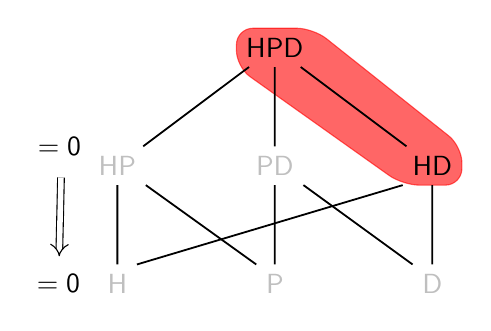
\begin{tikzpicture}[edge from parent/.style={draw,line width=0.65pt},
font=\sffamily\sansmath,
every node/.style={},level 1/.style={sibling distance=20mm},level 2/.style={sibling distance=10mm}
]
\node (HPD) {HPD}
    child { node (HP) {\textcolor{DimGray}{HP}}
      child { node (H) {\textcolor{DimGray}{H}} }
      %child { node (B) {B}  }
  }
    child { node (PD) {\textcolor{DimGray}{PD}}
      child { node (P) {\textcolor{DimGray}{P}}}
      %child { node (C) {C}}
  }
  child { node (HD) {\textcolor{black}{HD}}
      %child { node (BB) {B}}
      child { node (D) {\textcolor{DimGray}{D}}}
  };
  \draw[line width=0.65pt] (HP.south east) -- (P.north west);
  \draw[line width=0.65pt] (HD.south west) -- (H.north east);
  \draw[line width=0.65pt] (PD.south east) -- (D.north west);
  
  %% implies arrows
  \draw[implies-, double distance=2pt] ($(H.west) + (-0.49, 0.35)$) -- ($(HP.west) + (-0.355,-0.15)$);   
  
  
  \node at  ($(H.west) + (-0.5, 0)$) {$= 0$};
  \node at  ($(HP.west) + (-0.375,0.25)$) {$= 0$};
  
\begin{pgfonlayer}{background}
  %\draw[blue,fill=blue,opacity=0.6, rounded corners = 6pt]
  %(ABC.north west) -- (ABC.north east)  -- (AC.north east) -- (AC.south east) -- (C.south east) -- (C.south west)  -- (BC.south west) -- cycle  ;
  %\draw[red,fill=red,opacity=0.6, rounded corners = 6pt]  (HP.south west) -- (HP.north west) --
  %(HPD.north west) -- (HPD.north east)  -- (HPD.south east) -- (HP.south east)  -- cycle  ;
  \draw[red,fill=red,opacity=0.6, rounded corners = 6pt]  (HD.south east) -- (HD.north east) --
  (HPD.north east) -- (HPD.north west)  -- (HPD.south west) -- (HD.south west)  -- cycle  ;
\end{pgfonlayer}
\end{tikzpicture}
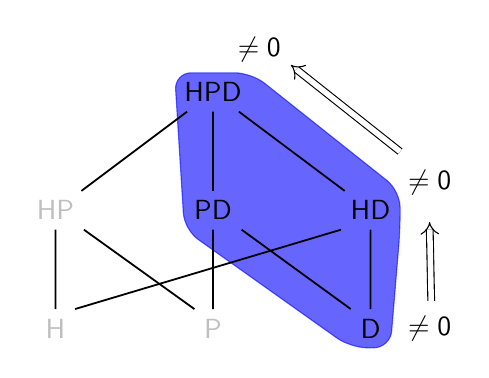
\begin{tikzpicture}[edge from parent/.style={draw,line width=0.65pt},
font=\sffamily\sansmath,
every node/.style={},level 1/.style={sibling distance=20mm},level 2/.style={sibling distance=10mm}
]
\node (HPD) {HPD}
    child { node (HP) {\textcolor{DimGray}{HP}}
      child { node (H) {\textcolor{DimGray}{H}} }
      %child { node (B) {B}  }
  }
    child { node (PD) {PD}
      child { node (P) {\textcolor{DimGray}{P}}}
      %child { node (C) {C}}
  }
  child { node (HD) {HD}
      %child { node (BB) {B}}
      child { node (D) {D}}
  };
  \draw[line width=0.65pt] (HP.south east) -- (P.north west);
  \draw[line width=0.65pt] (HD.south west) -- (H.north east);
  \draw[line width=0.65pt] (PD.south east) -- (D.north west);
  
  %% implies arrows
  \draw[-implies, double distance=2pt] ($(D.east) + (0.52, 0.35)$) -- ($(HD.east) + (0.375,-0.15)$); 
  
  \draw[implies-, double distance=2pt] ($(HPD.north east) + (0.5, 0.1)$) -- ($(HD.north east) + (0,0.5)$);   
  
  \node at  ($(D.east) + (0.5, 0)$) {$\neq 0$};
  \node at  ($(HD.east) + (0.375,0.35)$) {$\neq 0$};
  \node at  ($(HPD.north east) + (0.1, 0.3)$) {$\neq 0$};
  
\begin{pgfonlayer}{background}
  \draw[blue,fill=blue,opacity=0.6, rounded corners = 6pt]
  (HPD.north west) -- (HPD.north east)  -- (HD.north east) -- (HD.south east) -- (D.south east) -- (D.south west)  -- (PD.south west) -- cycle  ;
  %\draw[red,fill=red,opacity=0.6, rounded corners = 6pt]  (AB.south west) -- (AB.north west) --
  %(ABC.north west) -- (ABC.north east)  -- (ABC.south east) -- (AB.south east)  -- cycle  ;
\end{pgfonlayer}
\end{tikzpicture}
}
\vspace{5pt}


\end{center}
\end{document}
